\documentclass[aspectratio=43, 10pt]{beamer}

\usepackage[T2A]{fontenc}
\usepackage[utf8]{inputenc}
\usepackage[russian]{babel}
\usepackage{amsmath, amssymb, amsfonts}
\usepackage{booktabs}
\usepackage{graphicx}
\usepackage{tikz}
\usepackage{xcolor}
\usetikzlibrary{arrows.meta, positioning, shapes.geometric}

\usetheme{Madrid}
\usecolortheme{seahorse}
\setbeamertemplate{navigation symbols}{}
\setbeamertemplate{footline}[frame number]
\setbeamersize{text margin left=0.6cm, text margin right=0.6cm}

\graphicspath{
  {images/}
}

\newcommand{\R}{\mathbb{R}}
\newcommand{\E}{\mathbb{E}}
\newcommand{\KL}{\mathrm{KL}}
\newcommand{\Unif}{\mathrm{Unif}}
\newcommand{\cN}{\mathcal{N}}
\newcommand{\cB}{\mathcal{B}}

% --- Сквозная схема архитектуры: \archdiagram{<stage>} ---------------------
% stage = 1 -> активен только Encoder; 2 -> Encoder + Sinkhorn; 3 -> все блоки.
% Неактивные блоки рисуются бледными плейсхолдерами того же размера,
% поэтому положение схемы не меняется между слайдами.
\newcommand{\archdiagram}[1]{%
\resizebox{0.82\linewidth}{!}{%
\begin{tikzpicture}[
  active/.style={draw, rounded corners, minimum width=2.4cm, minimum height=0.9cm,
                 align=center, fill=blue!8},
  ghost/.style={draw=gray!40, dashed, rounded corners, minimum width=2.4cm,
                minimum height=0.9cm, align=center, fill=gray!4, text=gray!45},
  arron/.style={-{Latex[length=2mm]}, thick},
  arroff/.style={-{Latex[length=2mm]}, thick, gray!40}
]
  % --- блоки ---
  \node[active] (e) {Encoder\\$\Phi_\phi(x,y)$};
  \ifnum#1>1
    \node[active, below=0.65cm of e] (s) {Gumbel--Sinkhorn\\$Z\in\mathcal{B}_M$};
  \else
    \node[ghost, below=0.65cm of e] (s) {Gumbel--Sinkhorn};
  \fi
  \ifnum#1>2
    \node[active, below=0.65cm of s] (d) {Decoder\\$p_\theta(y\mid x)$};
  \else
    \node[ghost, below=0.65cm of s] (d) {Decoder};
  \fi
  % --- стрелки: тёмные только если оба соседних блока активны ---
  \ifnum#1>1
    \draw[arron] (e) -- node[right]{\small $\Phi$} (s);
  \else
    \draw[arroff] (e) -- node[right, gray!45]{\small $\Phi$} (s);
  \fi
  \ifnum#1>2
    \draw[arron] (s) -- node[right]{\small soft matching} (d);
  \else
    \draw[arroff] (s) -- node[right, gray!45]{\small soft matching} (d);
  \fi
\end{tikzpicture}
}}

\title[Восстановление парных зависимостей]{Восстановление парных зависимостей\\из групп непарных данных}
\author{Д.\,И.~Казачков}
\institute{МФТИ\\Научный руководитель: А.\,А.~Коротин}
\date{2026}

\begin{document}

% ============================================================
\begin{frame}
  \titlepage
\end{frame}

% ============================================================
% \begin{frame}{План}
% \begin{enumerate}
%   \item Постановка задачи и мотивация
%   \item Основной метод: CatVAE + Gumbel--Sinkhorn
%   \item Синтетический тор и метрики
%   \item Результаты экспериментов
%   \item Адаптация EM алгоритма
%   \item Выводы и ограничения
% \end{enumerate}
% \end{frame}

% ============================================================
\begin{frame}{Постановка задачи}
\begin{columns}[T]
\column{0.55\textwidth}
Есть $N$ независимых групп. В группе $n$ исходно были пары
\[
  (x^n_1, y^n_1), \dots, (x^n_M, y^n_M),
\]
но элементы $Y$ перемешаны неизвестной перестановкой $\sigma^n$:
\[
  \bigl\{x^n_m\bigr\}_{m=1}^{M},
  \qquad
  \bigl\{y^n_{\sigma^n(m)}\bigr\}_{m=1}^{M}.
\]

\vspace{0.4em}
Правдоподобие одной группы при латентной перестановке:
\[
  p(y^n \mid x^n)
  =
  \sum_{\sigma^n \in S_M}
  p(\sigma^n)
  \prod_{m=1}^{M}
  p(y^n_{\sigma^n(m)} \mid x^n_m).
\]

\column{0.43\textwidth}
\centering
\begin{tikzpicture}[
  xpt/.style={circle, fill=blue!70, inner sep=2.2pt},
  ypt/.style={circle, fill=orange!80, inner sep=2.2pt},
  arr/.style={-{Latex[length=2mm]}, thick, gray!70}
]
  \node[xpt, label=left:$x_1$] (x1) at (0, 2.2) {};
  \node[xpt, label=left:$x_2$] (x2) at (0, 1.2) {};
  \node[xpt, label=left:$x_3$] (x3) at (0, 0.2) {};
  \node[ypt, label=right:$y_1$] (y1) at (3, 2.0) {};
  \node[ypt, label=right:$y_2$] (y2) at (3, 0.4) {};
  \node[ypt, label=right:$y_3$] (y3) at (3, 1.2) {};
  \draw[arr, dashed] (x1) -- (y3);
  \draw[arr, dashed] (x2) -- (y2);
  \draw[arr, dashed] (x3) -- (y1);
  \node[align=center] at (1.5,-0.6) {\small неизвестная перестановка};
\end{tikzpicture}

\vspace{0.8em}
\begin{alertblock}{Комбинаторная сложность}
Сумма содержит $M!$ слагаемых. Уже при $M=20$ прямой подсчёт невозможен.
\end{alertblock}
\end{columns}
\end{frame}

% ============================================================
\begin{frame}{Мотивация}
Существующее решение (Beier et al.) --- заменить общую перестановку на совокупность независимых сопоставлений
\[
  \sigma^n(m) \in \{1,\dots,M\}.
\]

\vspace{-0.2em}
\[
  \sum_{\sigma^n} p(\sigma^n)\prod_{m=1}^{M} p \bigl(y^n_{\sigma^n(m)}\mid x^n_m\bigr)
  \quad \leadsto \quad
  \prod_{m=1}^{M}\sum_{\sigma^n(m)} p(\sigma^n(m))\,p \bigl(y^n_{\sigma^n(m)}\mid x^n_m\bigr).
\]

\begin{columns}[T]
\column{0.48\textwidth}
\begin{block}{Плюс}
Нет суммы по $M!$ перестановкам.
\end{block}

\column{0.48\textwidth}
\begin{alertblock}{Минус}
Биективность теряется: несколько $x_m$ могут выбрать один и тот же $y_k$.
\end{alertblock}
\end{columns}

\vspace{0.5em}
\textbf{Идея работы:} $\log p(y^n\mid x^n)$ оценить снизу вариационной
нижней оценкой и максимизировать уже её:
\[
  \log p(y^n\mid x^n)\;\ge\;\mathrm{ELBO}(\theta,\phi)
  \;\xrightarrow[\theta,\phi]{}\;\max,
\]
где перестановка $\sigma$ --- латентная переменная.
\end{frame}

% ============================================================
\begin{frame}{Posterior скрытой перестановки}
\small
Истинный posterior скрытой перестановки:
\[
  p_\theta(\sigma\mid x,y)
  =
  \frac{p_\theta(y,\sigma\mid x)}{p_\theta(y\mid x)}
  = 
  \dots
  =
  \frac{
  p(\sigma)\prod_{m=1}^{M}p_\theta(y_{\sigma(m)}\mid x_m)
  }{
  \sum_{\sigma'\in S_M}
  p(\sigma')\prod_{m=1}^{M}
  p_\theta(y_{\sigma'(m)}\mid x_m)
  }.
\]

\vspace{-0.2em}
\normalsize
Знаменатель всё ещё содержит $M!$ слагаемых. Вводим вариационное распределение на всём $S_M$:
\[
  q(\sigma\mid x,y)\ge 0,\qquad
  \sum_{\sigma\in S_M}q(\sigma\mid x,y)=1.
\]
\end{frame}

% ============================================================
\begin{frame}{ELBO и разрыв}
\footnotesize
\[
\begin{aligned}
  p_\theta(y\mid x)
  &=
  \sum_{\sigma\in S_M}q(\sigma)
  \frac{p_\theta(y,\sigma\mid x)}{q(\sigma)} 
  \Rightarrow  \log p_\theta(y\mid x) \ge  \E_q\left[  \log\frac{p_\theta(y,\sigma\mid x)}{q(\sigma)}  \right]  :=\mathcal{E}(q,\theta;x,y),\\
  \mathcal{E}(q,\theta;x,y)
  &=
  \E_q\left[
    \log p_\theta(y,\sigma\mid x)-\log q(\sigma)
  \right]\\
  &=
  \E_{q(\sigma\mid x,y)}
  \left[
    \sum_{m=1}^{M}
    \log p_\theta(y_{\sigma(m)}\mid x_m)
  \right]
  -
  \KL\!\left(
    q(\sigma\mid x,y)\,\middle\|\,\Unif(S_M)
  \right).
\end{aligned}
\]

\vspace{-0.4em}
\[
\boxed{
\begin{aligned}
  \mathcal L_{\mathrm{NELBO}}(\theta,q)
  &=
  \frac{1}{N}\sum_{n=1}^{N}
  \left[
  \E_{q_n}
  \left[
  -\sum_{m=1}^{M}\log p_\theta(y^n_{\sigma(m)}\mid x^n_m)
  \right]
  +
  \KL\!\left(q_n(\sigma)\,\middle\|\,\Unif(S_M)\right)
  \right].
\end{aligned}
}
\]

% \vspace{-0.5em}
\footnotesize

Но это в предположении $p(\sigma)\sim\Unif(S_M)$. А с истинным posterior как это соотносится?
\[
\boxed{
  \log p_\theta(y\mid x)
  =
  \mathcal{E}(q,\theta;x,y)
  +
  \KL\!\left(
  q(\sigma\mid x,y)\,\middle\|\,p_\theta(\sigma\mid x,y)
  \right).
}
\]

\vspace{-0.3em}
\footnotesize
Максимизируем $\mathcal{E}(q,\theta)$.

\vspace{0.3em}
\begin{block}{}
\centering
Как представить и оптимизировать $q(\sigma\mid x,y)$? Как параметризовать $p_\theta(y\mid x)$?
\end{block}
\end{frame}

% ============================================================
\begin{frame}{Нейросетевой вариационный подход}
\small
Два распределения параметризуются нейросетями и обучаются совместно:

\vspace{0.3em}
\begin{itemize}
  \setlength{\itemsep}{0.5em}
  \item $q_\phi(\sigma\mid x,y)$ задаётся энкодером и Gumbel--Sinkhorn-релаксацией
        мягкой матрицы перестановки $Z\in\mathcal{B}_M$.
  \item $p_\theta(y\mid x)$ задаётся декодером как условная wrapped Gaussian mixture.
  \item Точный KL на $S_M$ недоступен для Gumbel--Sinkhorn-распределения, поэтому в
        реализации используется дифференцируемый surrogate loss.
\end{itemize}

\vspace{0.2em}
\[
\begin{aligned}
  D^n_{mk}&=-\log p_\theta(y^n_k\mid x^n_m),\\
  \mathcal{L}^n
  &=
  \sum_{m,k}z^n_{mk}D^n_{mk}
  +\beta\,\frac{1}{M}\sum_{m,k}z^{n,\mathrm{det}}_{mk}
  \bigl(\log z^{n,\mathrm{det}}_{mk}+\log M\bigr).
\end{aligned}
\]
\end{frame}

% ============================================================
\begin{frame}{CatVAE: энкодер}
\small
\begin{columns}[T]
\column{0.5\textwidth}
\textbf{Энкодер} по \emph{всем} парам $(x^n_m,y^n_k)$ строит матрицу логитов:
\[
\begin{aligned}
  \Phi_{mk}
\!=\!
  f_\phi\!\bigl([
    \sin 2\pi x^n_m,\cos 2\pi x^n_m,\\
    \sin 2\pi y^n_k,\cos 2\pi y^n_k
  ]\bigr).
\end{aligned}
\]

\vspace{-0.1em}
Если нормировать только строки, получится локальное распределение кандидатов:
\[
  \Pr(k\mid m)
  =
  \frac{\exp(\Phi_{mk})}{\sum_{k'=1}^{M}\exp(\Phi_{mk'})}.
\]

\vspace{0.3em}
Но это только мотивационный промежуточный вариант: построчная нормировка
\emph{не} гарантирует биективность, так как несколько $x_m$ могут выбрать один $y_k$.

\column{0.38\textwidth}
\centering
\archdiagram{1}
\end{columns}
\end{frame}

% ============================================================
\begin{frame}{CatVAE: преобразование в латентном пространстве}
\small
\textbf{Энкодер} выдаёт логиты
$\Phi_{mk}=f_\phi([\sin 2\pi x_m,\cos 2\pi x_m,\sin 2\pi y_k,\cos 2\pi y_k])
\in\mathbb{R}^{M\times M}$. В общем случае эта матрица \emph{не} перестановочна;
превращаем её в мягкую перестановку $Z\in\cB_M$.

\vspace{0.5em}
\textbf{1. Gumbel trick:} добавляем шум и делим на температуру $\tau$
\[
  \tilde \Phi_{mk}
  =
  \frac{\Phi_{mk}+G_{mk}}{\tau},
  \qquad
  G_{mk}\sim \mathrm{Gumbel}(0,1).
\]

\vspace{0.4em}
\textbf{2. Sinkhorn-Knopp в log-space:} последовательно нормируем строки и столбцы
\[
  \tilde \Phi^{(t+\frac12)}_{mk}
  =
  \tilde \Phi^{(t)}_{mk}
  -
  \log\sum_{j=1}^{M}\exp \tilde \Phi^{(t)}_{mj},
  \qquad
  \tilde \Phi^{(t+1)}_{mk}
  =
  \tilde \Phi^{(t+\frac12)}_{mk}
  -
  \log\sum_{i=1}^{M}\exp \tilde \Phi^{(t+\frac12)}_{ik}.
\]

\vspace{0.4em}
Тогда матрица сопоставлений определяется так:
\[
  Z=\exp(\tilde \Phi^{(T)})\in\cB_M,\qquad
  Z_{mk}\ge 0,\quad
  \sum_k Z_{mk}\approx 1,\quad
  \sum_m Z_{mk}\approx 1.
\]
\end{frame}

% ============================================================
\begin{frame}{CatVAE: преобразование в латентном пространстве}
\small
\begin{columns}[T]
\column{0.6\textwidth}
\textbf{Энкодер} выдаёт логиты $\Phi_{mk}=f_\phi(\dots)$. \\
\textbf{Gumbel--Sinkhorn} переводит логиты в матрицу сопоставлений $Z\in\cB_M$.

\vspace{0.6em}
\begin{itemize}
  \setlength{\itemsep}{0.5em}
  \item $Z_{mk}$ задает степень соответствия $x_m$ и $y_k$.
  \item Дважды стохастическая $Z$ задает релаксацию биективного сопоставления.
  \item Температура $\tau$: большая --- масса распределяется более равномерно по строкам и столбцам; 
        малая --- $Z$ близка к разреженной дважды стохастической матрице.
  \item В основных экспериментах $\tau=1$ фиксирована на протяжении запуска.
  \item Операция дифференцируема $\Rightarrow$ энкодер обучается end-to-end
        градиентами через $Z$.
\end{itemize}

\column{0.38\textwidth}
\centering
\archdiagram{2}
\end{columns}
\end{frame}

% ============================================================
\begin{frame}{Декодер: wrapped Gaussian mixture}
\small
\begin{columns}[T]
\column{0.7\textwidth}
\textbf{Энкодер} выдает логиты $\Phi_{mk}=f_\phi(\dots)$. \\
\textbf{Gumbel--Sinkhorn} выдает матрицу сопоставлений $Z\in\cB_M$.

\vspace{0.4em}
\textbf{Декодер} задаёт условную плотность как смесь $K$ компонент:
\[
  p_\theta(y\mid x)
  =
  \sum_{c=1}^{K}
  \pi_c(x)\,
  \widetilde{\cN}\!\left(y\mid \mu_c(x),\epsilon^2\right).
\]

\vspace{0.3em}
\begin{itemize}
  \item $\mu_c(x)$ и logits для $\pi_c(x)$ выдаёт MLP по признакам
        $[\sin(2\pi x),\cos(2\pi x)]$; его обучаемые веса --- это параметры $\theta$.
  \item $\widetilde{\cN}$ --- гауссовская плотность, обёрнутая на тор через $z\mapsto z\bmod 1$.
  \item $\epsilon^2$ фиксирована и совпадает с дисперсией шума генератора.
  \item Для синтетических экспериментов используется $K=2$.
\end{itemize}

\column{0.38\textwidth}
\centering
\archdiagram{3}
\end{columns}
\end{frame}

% ============================================================
\begin{frame}{Синтетические данные на торе}
\begin{columns}[T]
\column{0.5\textwidth}
Работаем на $S^1=[0,1)$:
\[
  P_{\mathrm{data}}(x) := \mathcal{U}[0,1), \qquad X\in[0,1),
\]
\[
  P_{\mathrm{data}}(y\mid x)
  :=
  \frac{1}{2}\widetilde{\cN}(x,\epsilon^2)
  +
  \frac{1}{2}\widetilde{\cN}(x+0.3,\epsilon^2).
\]

\vspace{0.4em}
После генерации пар внутри каждой группы элементы $Y$ перемешиваются случайной перестановкой.

\column{0.46\textwidth}
\centering
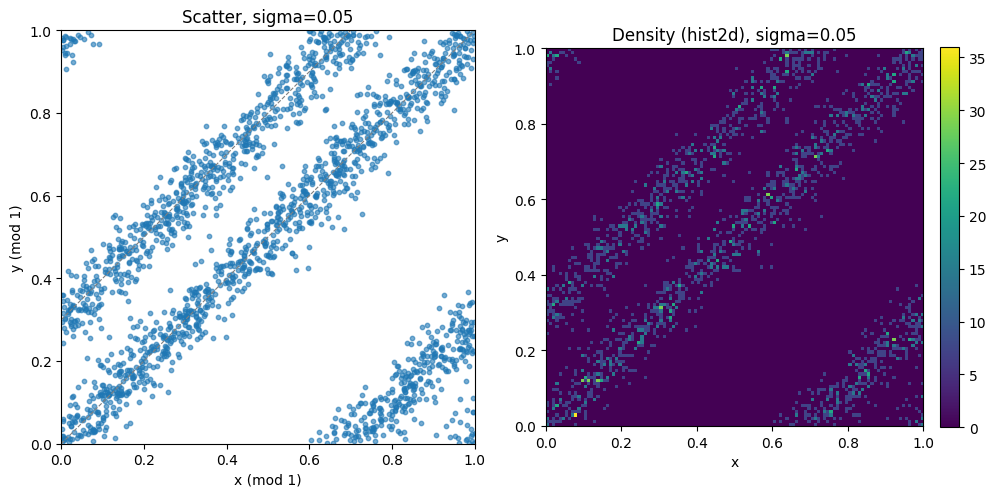
\includegraphics[width=\linewidth]{data_orig_generation_torus.png}

\vspace{0.2em}
{\footnotesize Две диагональные полосы: $y\approx x$ и $y\approx x+0.3$.}
\end{columns}

\begin{block}{Метрика восстановления плотности}
Так как $X\sim \mathcal{U}[0,1)$, \(p(x,y)=p(y\mid x)\). На сетке $E\times E$ считаем
\[
  L_2
  =
  \frac{1}{E}
  \left\|
    p_{\mathrm{true}}(x,y)-\widehat p_\theta(x,y)
  \right\|_2,
  \qquad E=100.
\]
\end{block}
\end{frame}

% ============================================================
\begin{frame}{Эксперимент 1: влияние размера группы $M$}
\centering
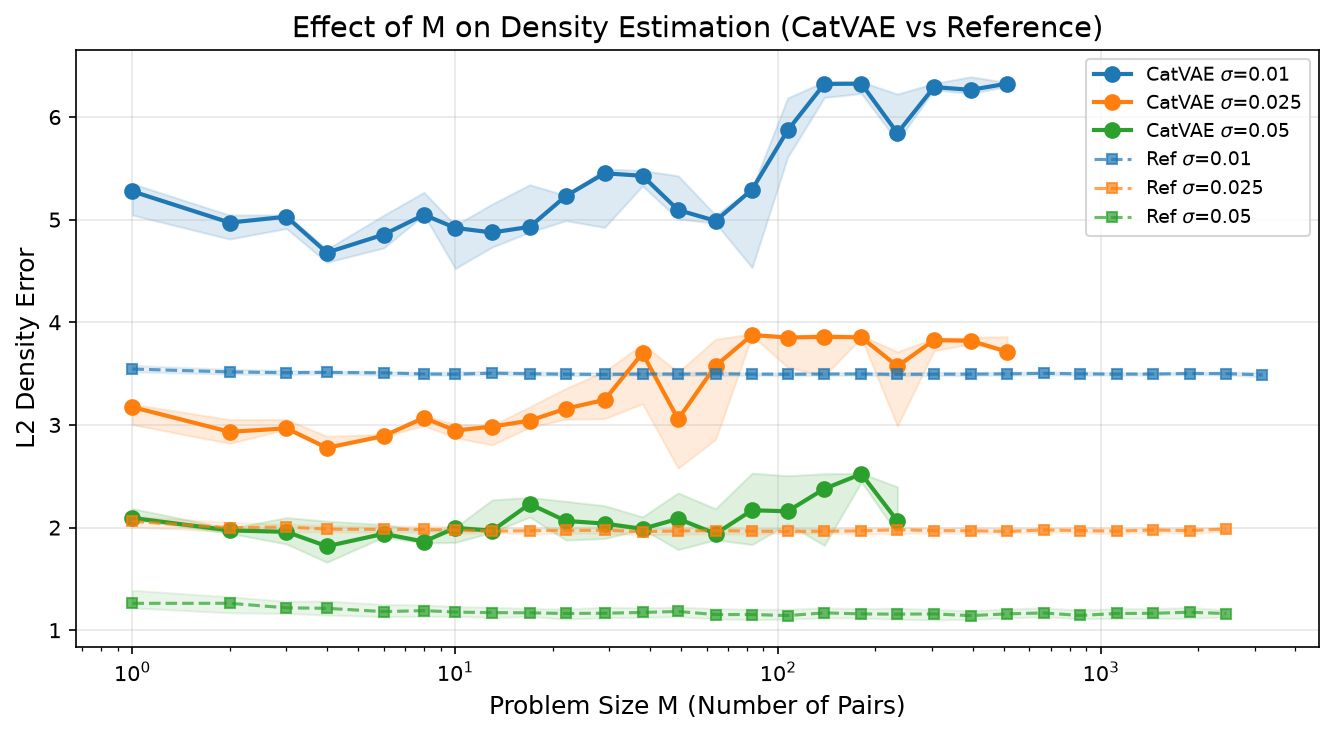
\includegraphics[height=0.58\textheight]{varying_M_sgd_spread.png}

\vspace{-0.4em}
\small
\begin{itemize}
  \item Рост $M$ увеличивает пространство перестановок как $M!$.
  \item Для малых $M$ плотность восстанавливается конкурентно.
  \item При больших $M$ bottleneck переходит в качество matching/энкодера.
\end{itemize}
\end{frame}

% ============================================================
\begin{frame}{Эксперимент 2: влияние объёма данных $N$}
\centering
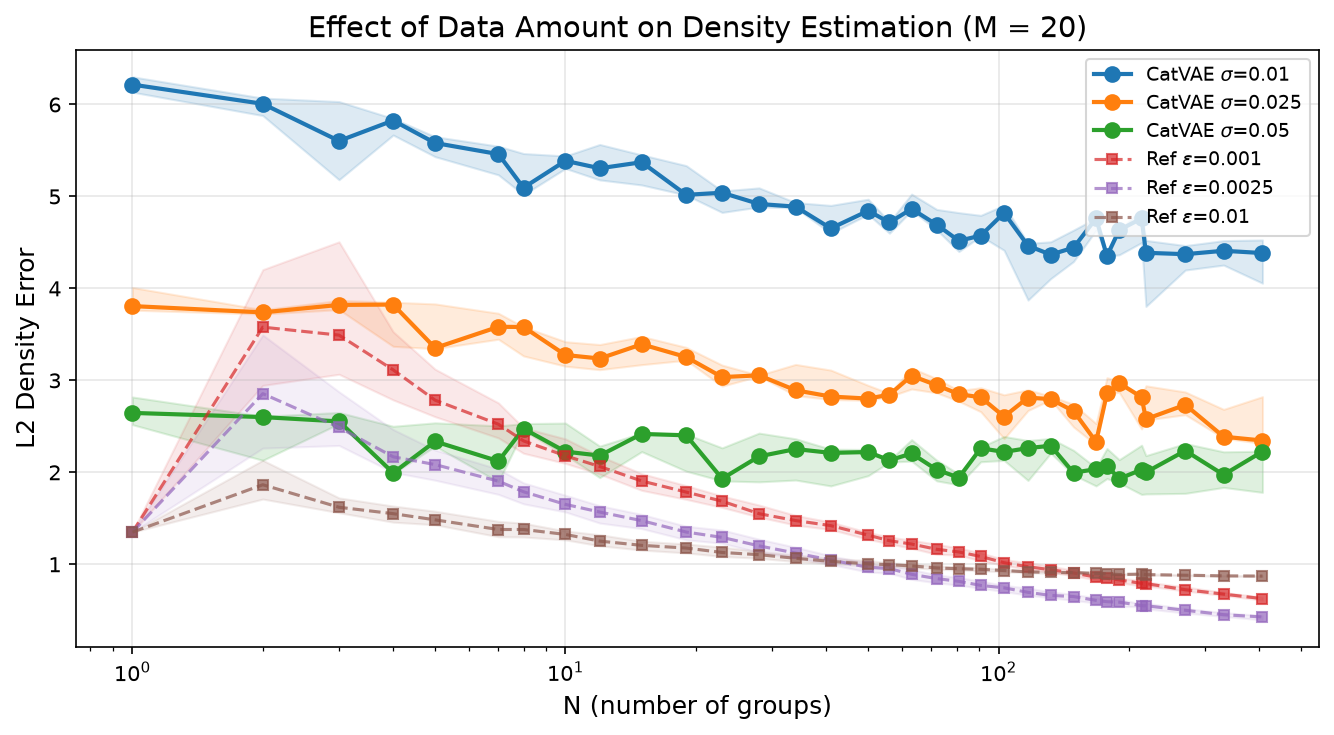
\includegraphics[height=0.58\textheight]{varying_N_sgd_spread.png}

\vspace{-0.4em}
\small
\begin{itemize}
  \item Увеличение числа групп помогает оценке плотности, но не решает полностью matching-задачу.
  \item Для больших $M$ важна не только статистика, но и архитектура inference-модели.
\end{itemize}
\end{frame}

% ============================================================
\begin{frame}{Эксперимент 3: сравнение восстановления плотности}
  \centering
  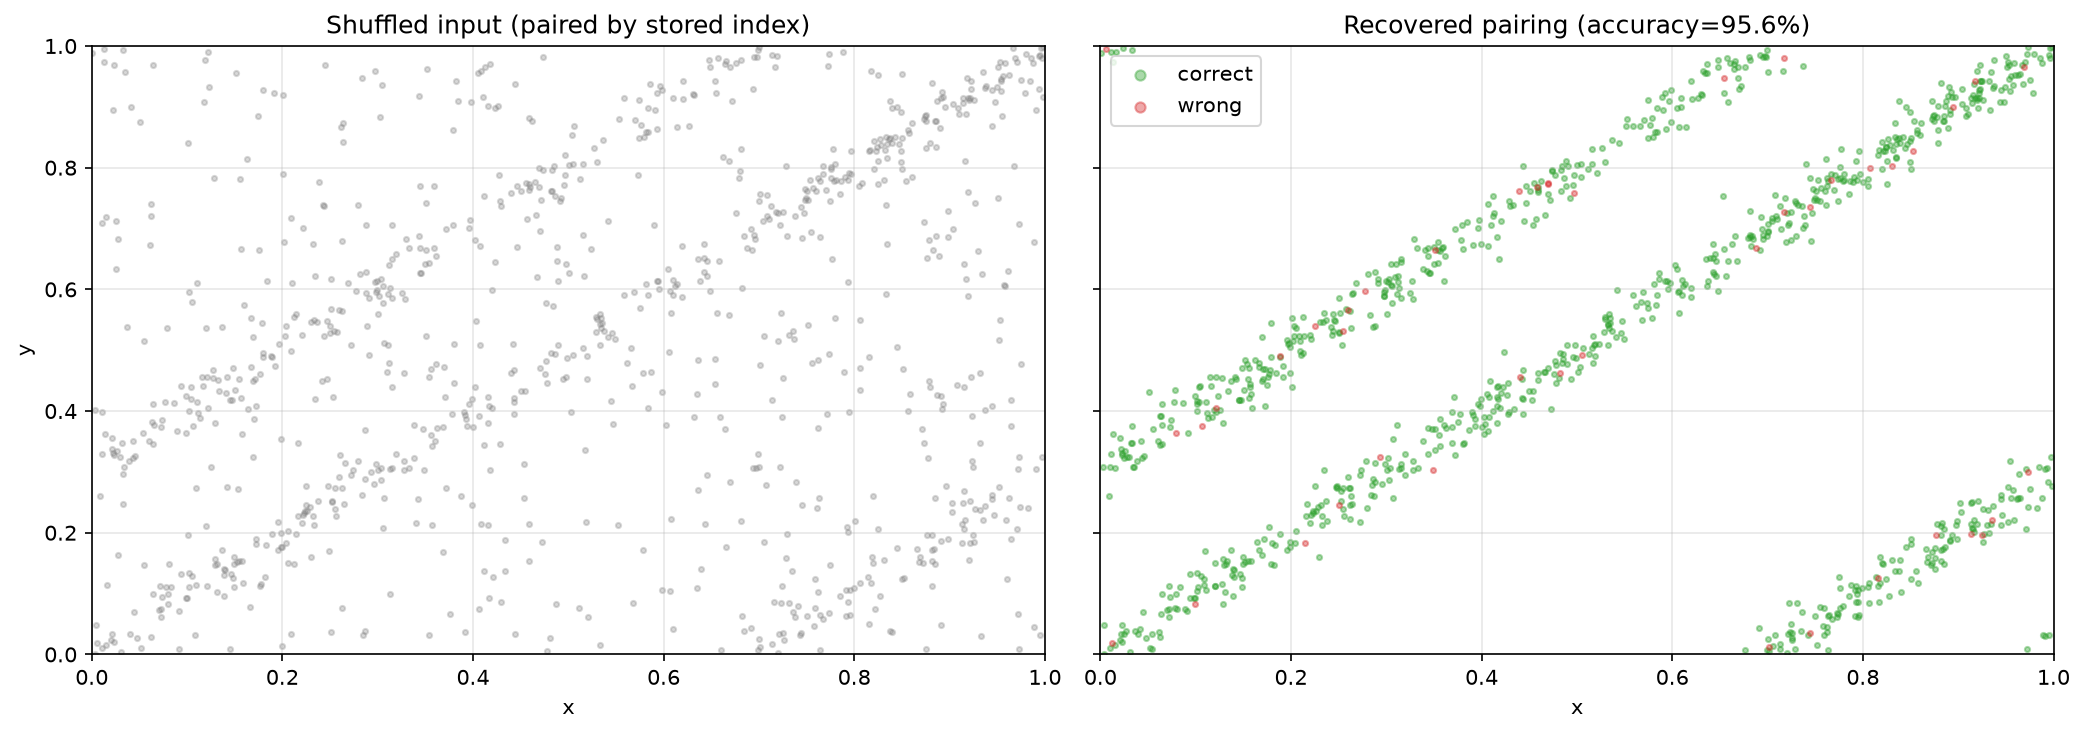
\includegraphics[width=0.64\textwidth]{sigma_0.025_sgd_spread_recovery.png}\\
  {\footnotesize $\epsilon=0.025$, $M=2$}

  \vspace{0.1em}
  \begin{minipage}{0.42\textwidth}
    \centering
    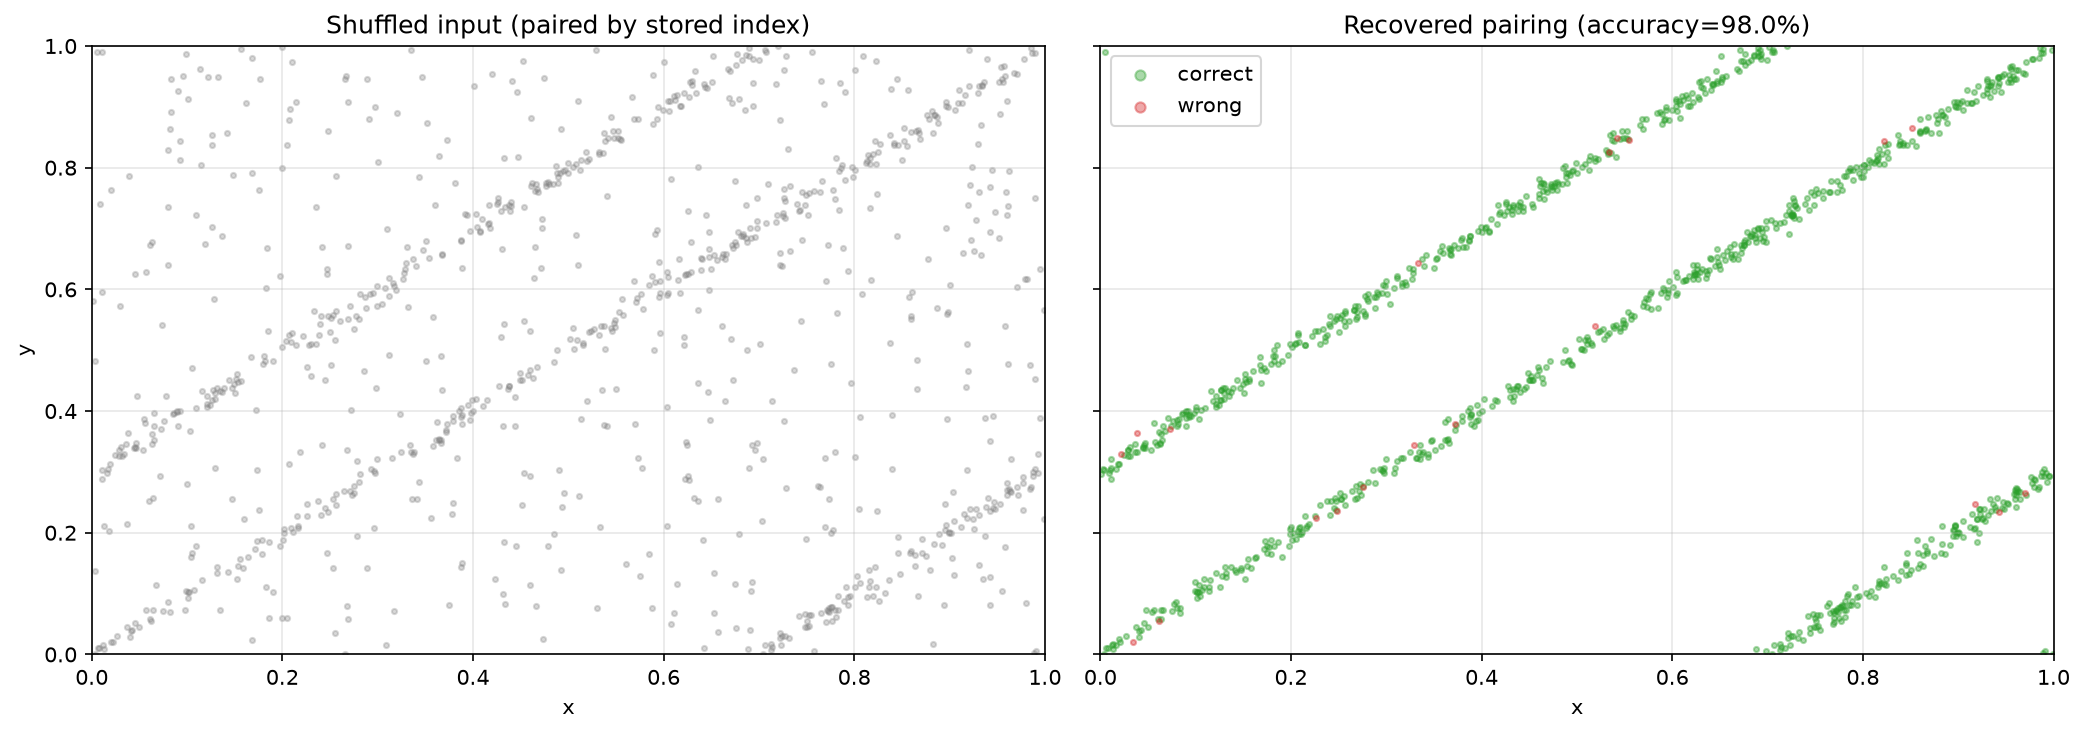
\includegraphics[width=\linewidth]{sigma_0.01_sgd_spread_recovery.png}\\
    {\footnotesize $\epsilon=0.01$, $M=2$}
  \end{minipage}\hfill
  \begin{minipage}{0.42\textwidth}
    \centering
    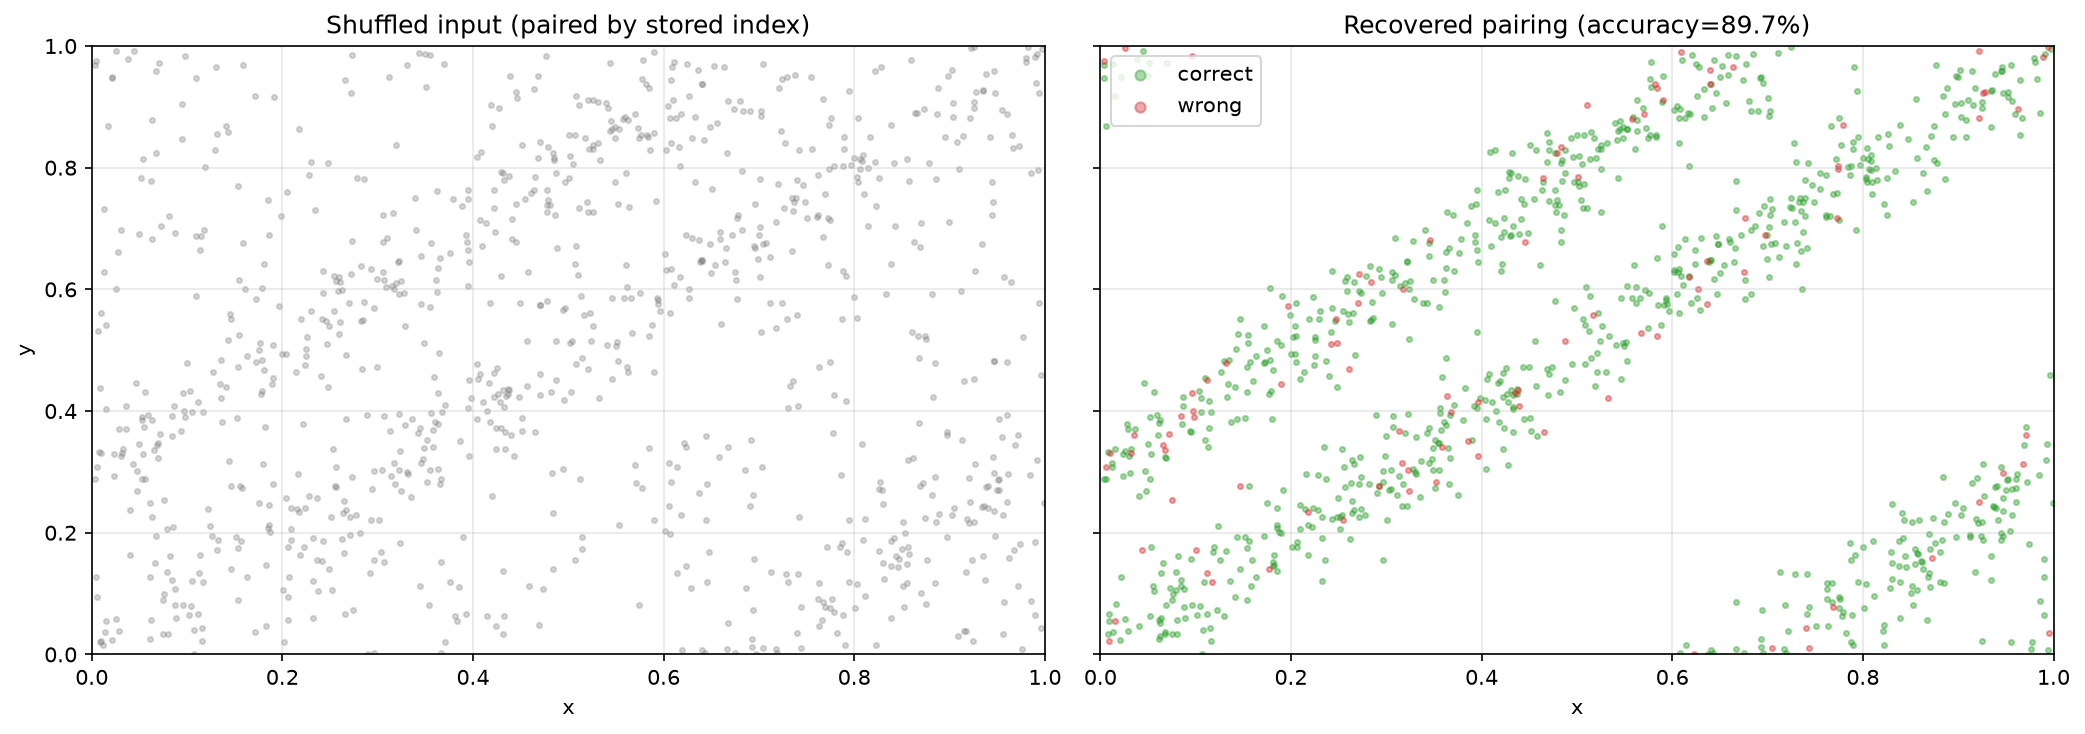
\includegraphics[width=\linewidth]{sigma_0.05_sgd_spread_recovery.png}\\
    {\footnotesize $\epsilon=0.05$, $M=2$}
  \end{minipage}

  \vspace{0.6em}
  \centering
  \begin{minipage}{\textwidth}
  \small
  \begin{itemize}
    \item Модель восстанавливает периодичность и диагональную структуру.
    \item При росте $\epsilon$ моды сильнее перекрываются, matching становится неоднозначнее.
    \item Для малых групп accuracy существенно выше случайного baseline.
  \end{itemize}
  \end{minipage}
  \end{frame}

% ============================================================
\begin{frame}{EM: вероятностная модель}
\small
К условному распределению
\[
  p_\theta(y\mid x)
  =
  \sum_{c=1}^{K}
  \pi_c\,
  \widetilde{\cN}\!\left(y\mid x+s_c,\epsilon^2\right),
\]
с параметрами $\theta=(\pi_1,\ldots,\pi_K,s_1,\ldots,s_K)$ 
добавляется набор скрытых переменных $c_m\in\{1,\dots,K\}$. Тогда вероятностная модель:
\[
  p_\theta(y,\sigma,c\mid x)
  =
  p(\sigma)
  \prod_{m=1}^{M}
  \pi_{c_m}
  \widetilde{\mathcal N}
  \left(
  y_{\sigma(m)}
  \mid
  x_m+s_{c_m},
  \epsilon^2
  \right).
\]
\end{frame}

% ============================================================
\begin{frame}{EM: E-шаг}
\small
При текущих параметрах $\theta^{(t)}$ для каждой пары вычисляется лог-правдоподобие пары
\[
  L_{mk}
  =
  \log p_{\theta^{(t)}}(y_k\mid x_m)
  =
  \log\sum_{c=1}^{K}
  \pi_c^{(t)}\,
  \widetilde{\cN}\!\left(y_k\mid x_m+s_c^{(t)},\epsilon^2\right).
\]

\vspace{0.5em}
\begin{columns}[T]
\column{0.34\textwidth}
насколько вероятно, что $x_m$ соответствует $y_k$
\column{0.62\textwidth}
\[
  Q=\operatorname{Sinkhorn}\!\left(\frac{L}{\tau}\right).
\]
\end{columns}

\vspace{0.5em}
\begin{columns}[T]
\column{0.34\textwidth}
если $(x_m,y_k)$, то какая компонента $c$ объясняет эту пару?
\column{0.62\textwidth}
\[
  W_{mkc}
  =
  \frac{
    \pi_c\,\widetilde{\cN}\!\left(y_k\mid x_m+s_c,\epsilon^2\right)
  }{
    \sum_{c'}\pi_{c'}\,\widetilde{\cN}\!\left(y_k\mid x_m+s_{c'},\epsilon^2\right)
  }
\]
\end{columns}

\vspace{4em}
Совместный приближённый вес считается как
\[
  R_{mkc}=Q_{mk}W_{mkc}.
\]
Эту формулу можно понимать $R_{mkc}\approx\Pr[\sigma(m)=k,\ c_m=c\mid x,y,\theta]$.

\end{frame}

% ============================================================
\begin{frame}{EM: M-шаг}
\small
Обновление весов смеси
\[
  \pi_c
  \leftarrow
  \frac{S_c}{\sum_{c'}S_{c'}},
  \qquad
  S_c
  =
  \sum_{n,m,k}
  R^{(n)}_{mkc}.
\]

\vspace{0.6em}
Обновление сдвигов компонент
\[
  s_c
  \leftarrow
  \frac1{2\pi}
  \operatorname{atan2}\!\left(
    \sum_{n,m,k}
    R^{(n)}_{mkc}
    \sin(2\pi\delta^n_{mk}),\;
    \sum_{n,m,k}
    R^{(n)}_{mkc}
    \cos(2\pi\delta^n_{mk})
  \right)
  \bmod 1
\]
\end{frame}

% ============================================================
\begin{frame}{EM: эксперименты при $\tau=1$}
\begin{columns}[T]
\column{0.5\textwidth}
\centering
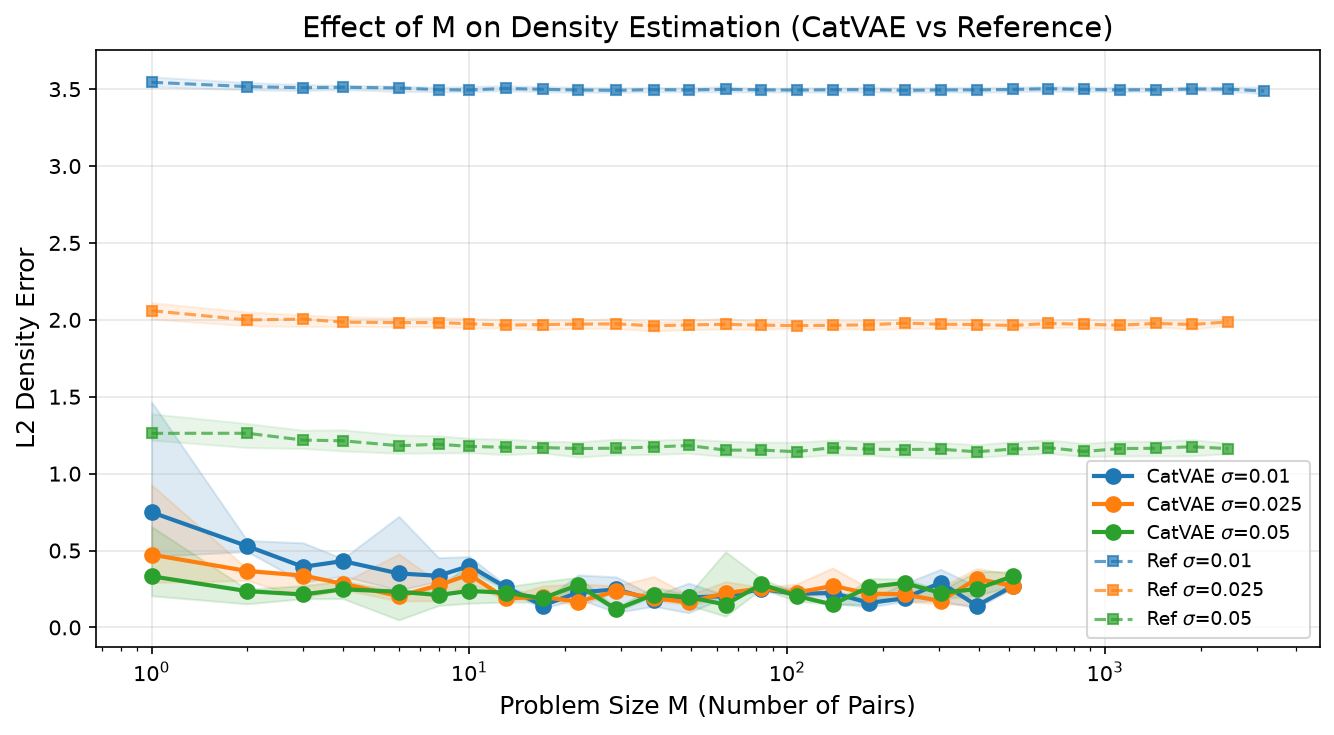
\includegraphics[width=\linewidth]{varying_M_em_tau1.0.png}\\
{\footnotesize EM: зависимость $L_2$ от $M$}

\column{0.5\textwidth}
\centering
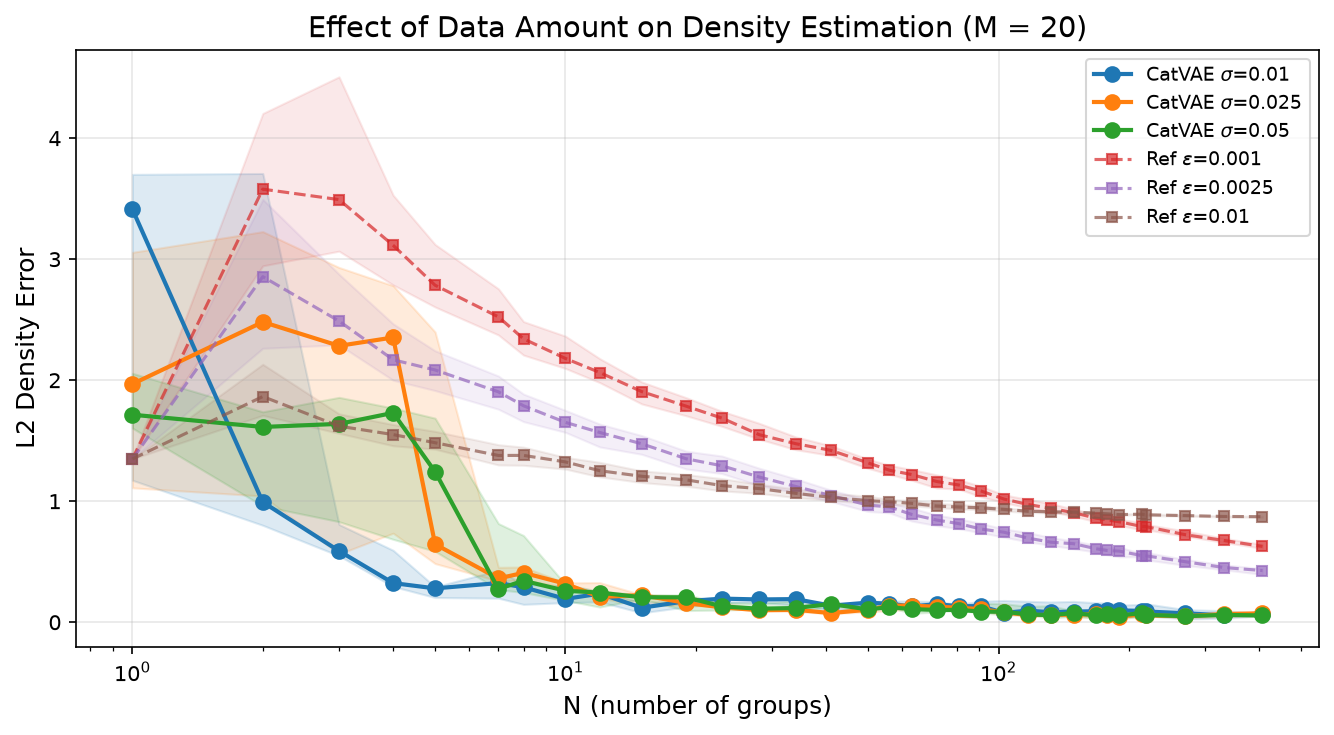
\includegraphics[width=\linewidth]{varying_N_em_tau1.0.png}\\
{\footnotesize EM: зависимость $L_2$ от $N$}
\end{columns}

\vspace{0.5em}
\begin{itemize}
  \item При $\tau=1$ ошибка смеси сдвигов не растёт с увеличением $M$ в исследованном диапазоне.
  \item С ростом $N$ параметры сдвигов и весов оцениваются точнее, ошибка стремится к малым значениям.
  \item Преимущество связано с правильно специфицированной моделью генератора.
\end{itemize}
\end{frame}

% ============================================================
\begin{frame}{EM: чувствительность к температуре}
\centering
\begin{tabular}{@{}cccc@{}}
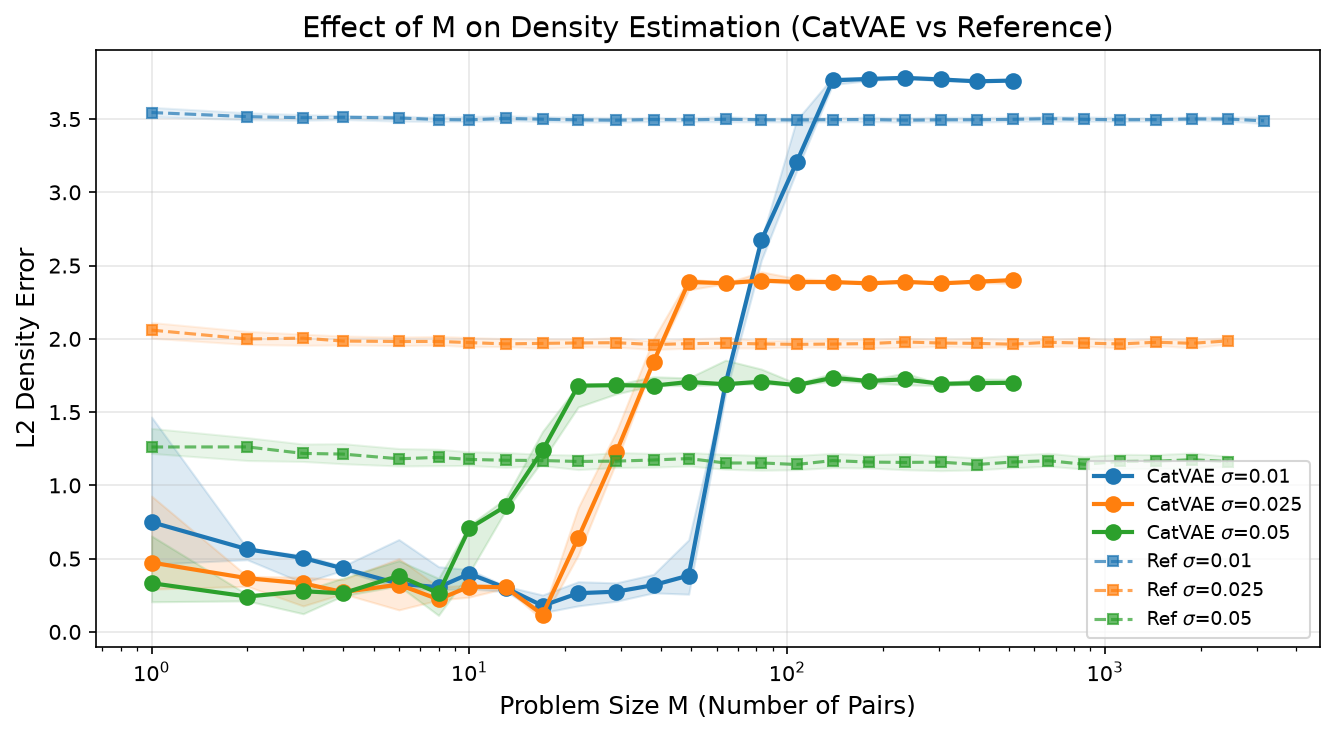
\includegraphics[width=0.235\textwidth]{varying_M_em_tau0.05.png} &
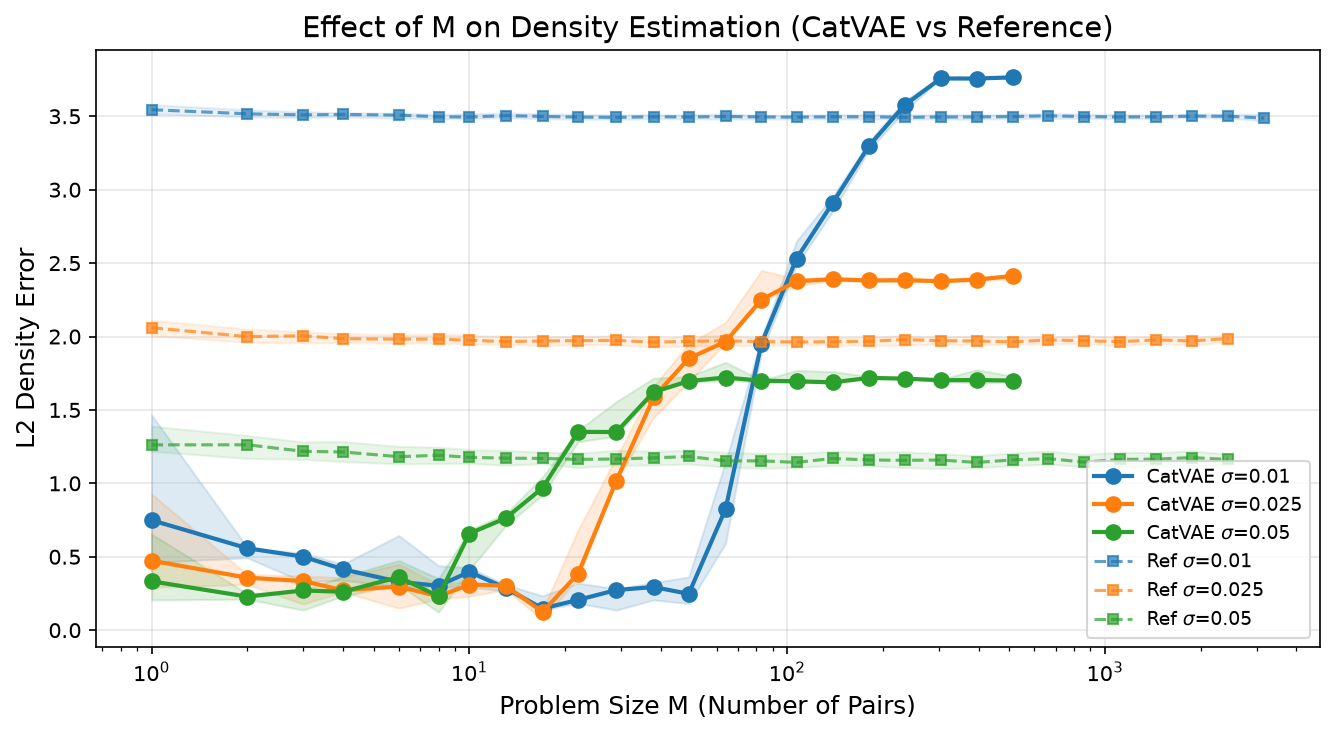
\includegraphics[width=0.235\textwidth]{varying_M_em_tau0.1.png} &
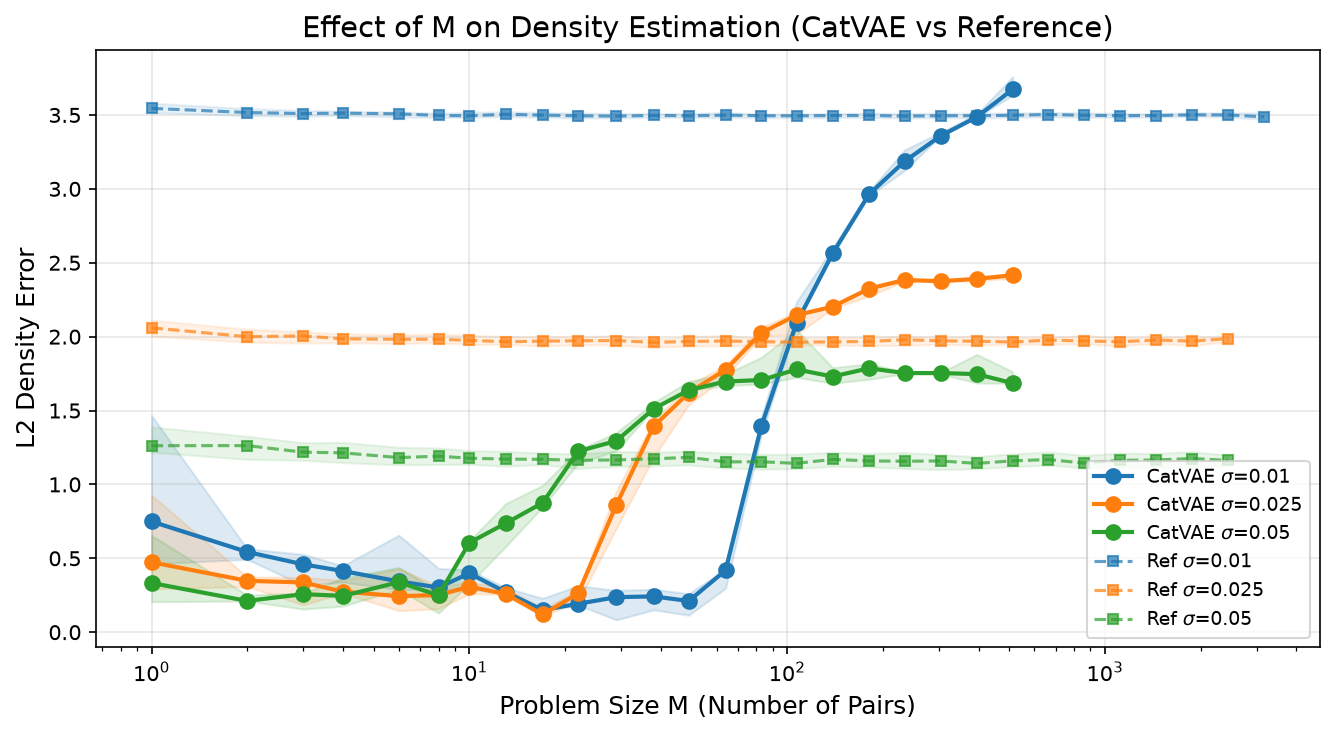
\includegraphics[width=0.235\textwidth]{varying_M_em_tau0.2.png} &
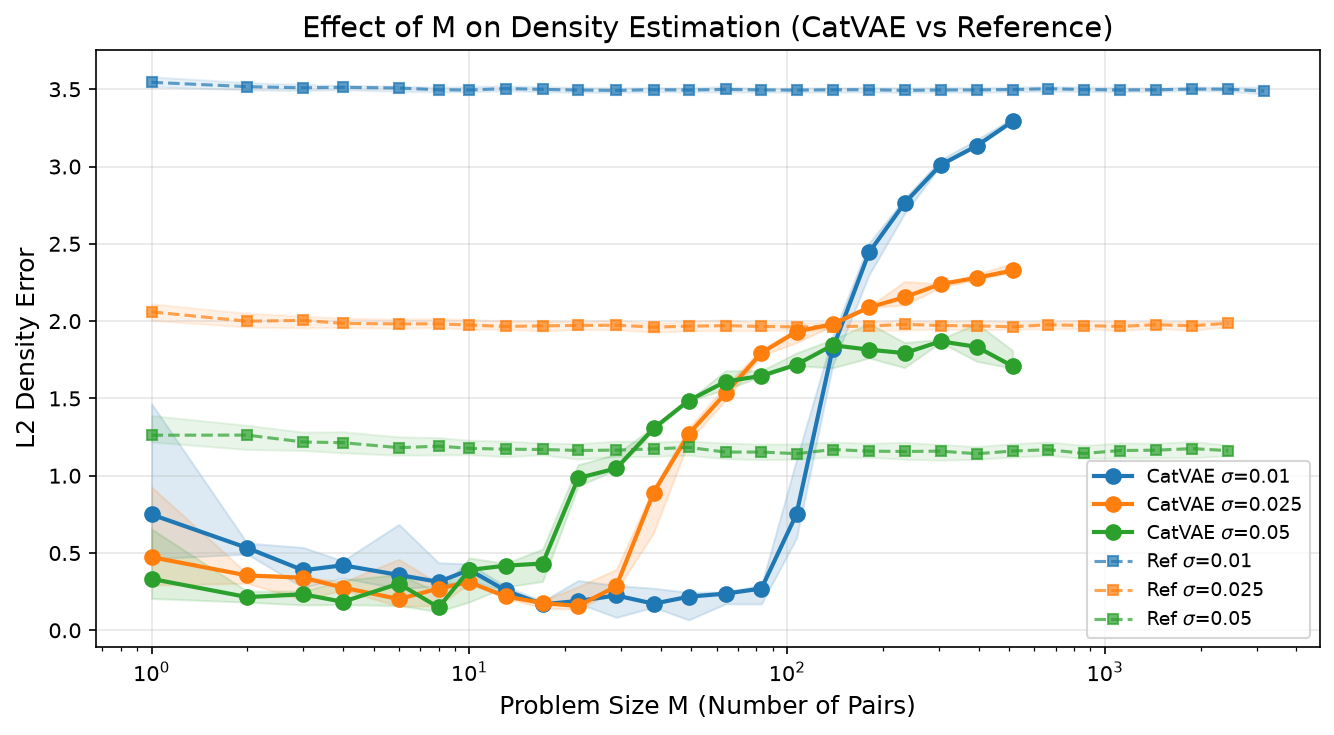
\includegraphics[width=0.235\textwidth]{varying_M_em_tau0.5.png} \\
{\footnotesize $\tau=0.05$} & {\footnotesize $\tau=0.1$} &
{\footnotesize $\tau=0.2$} & {\footnotesize $\tau=0.5$} \\[-0.1em]
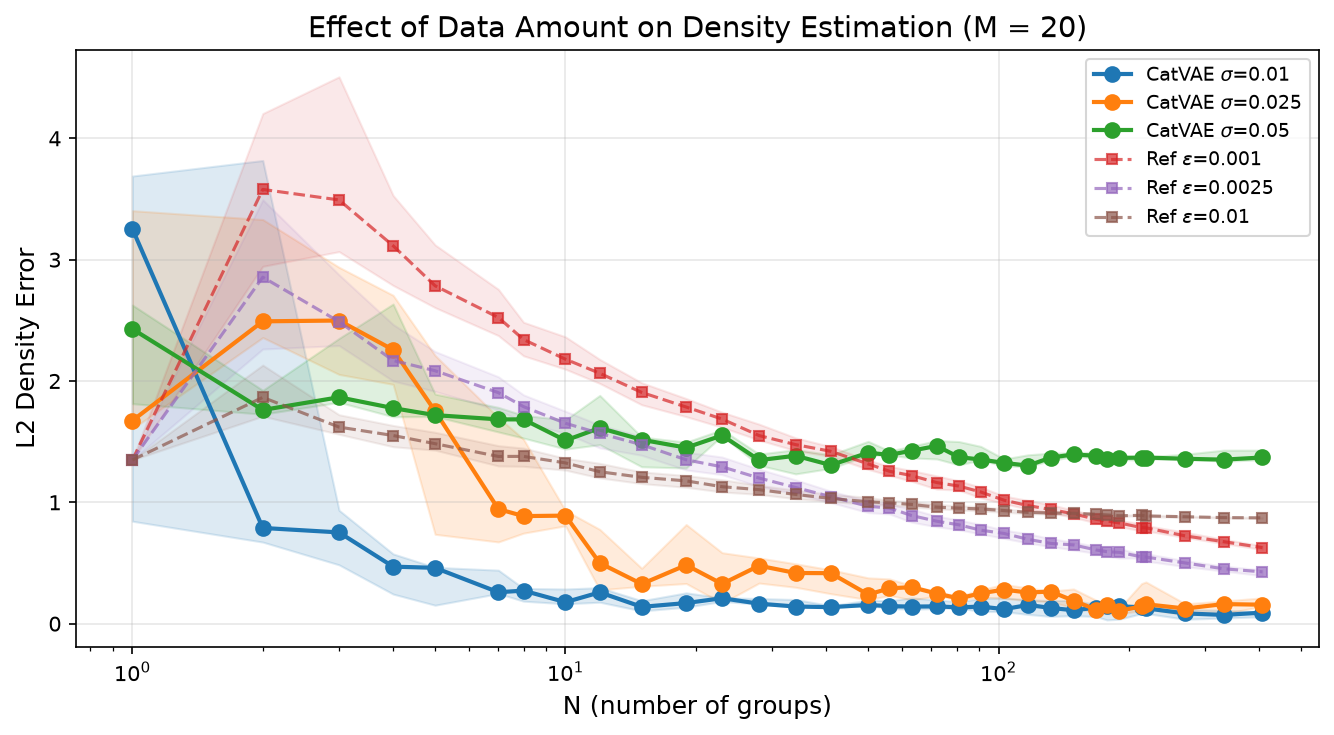
\includegraphics[width=0.235\textwidth]{varying_N_em_tau0.05.png} &
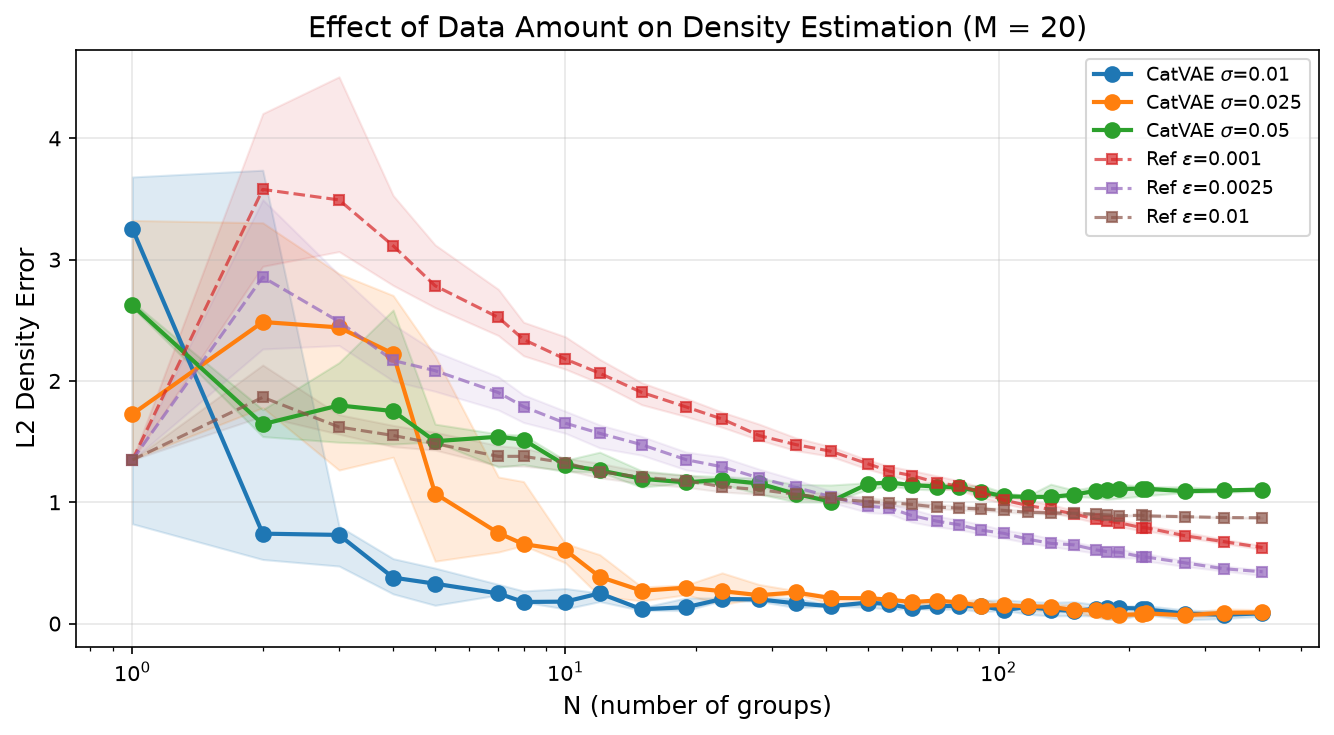
\includegraphics[width=0.235\textwidth]{varying_N_em_tau0.1.png} &
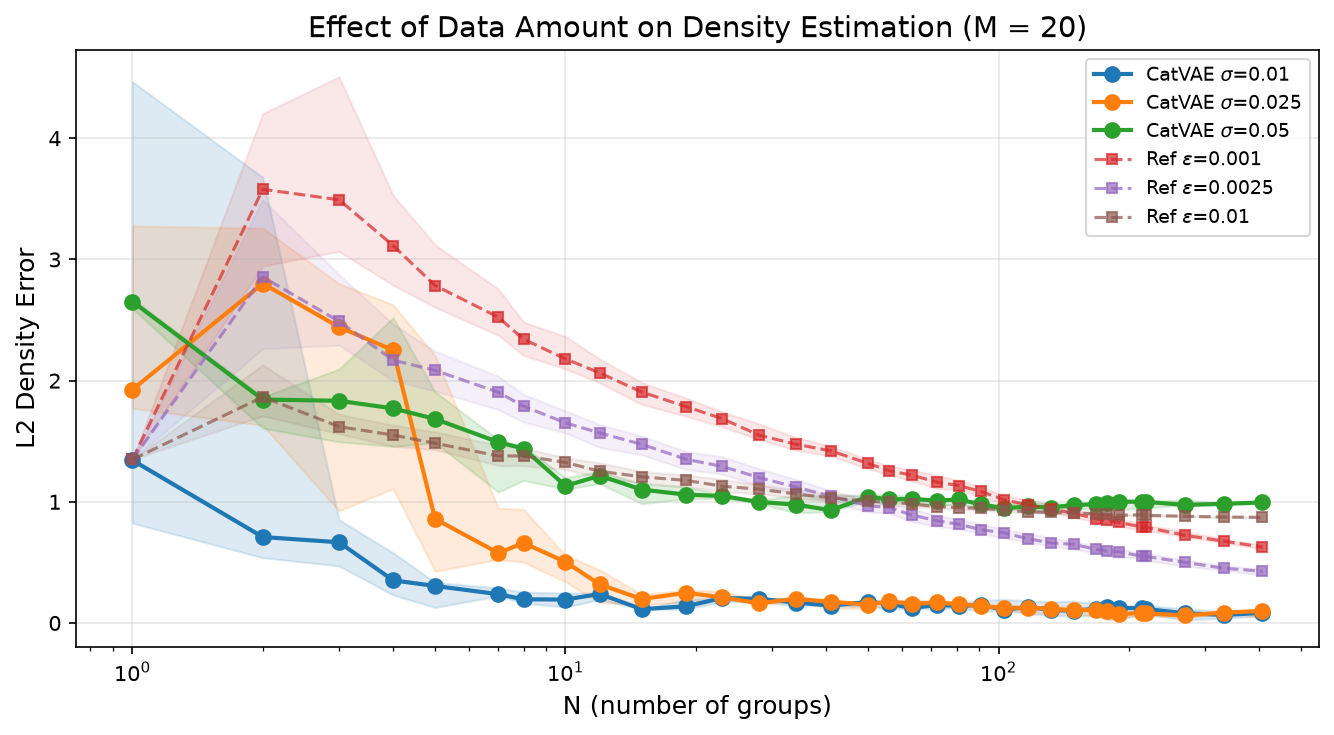
\includegraphics[width=0.235\textwidth]{varying_N_em_tau0.2.png} &
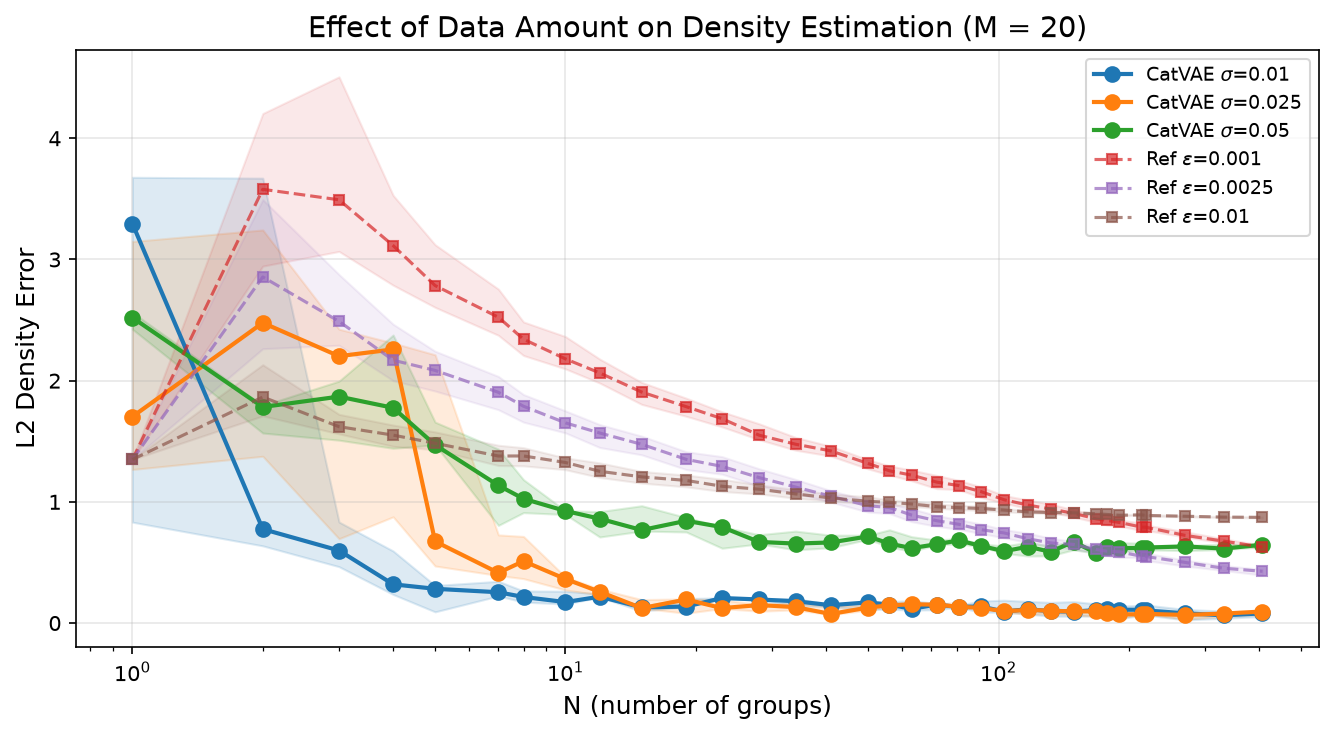
\includegraphics[width=0.235\textwidth]{varying_N_em_tau0.5.png}
\end{tabular}

\vspace{0.25em}
\small
При малой $\tau$ Sinkhorn-план становится почти жёстким:
ответственность может схлопнуться в одну компоненту, поэтому возникает плато ошибки.
\end{frame}

% ============================================================
\begin{frame}{Выносится на защиту}
\begin{enumerate}
  \item Выведена вариационная нижняя граница для точной скрытой перестановки группы, без факторизации по локальным назначениям.
  \item Разработан CatVAE с Gumbel--Sinkhorn-энкодером и декодером условной обёрнутой гауссовой смеси; модель амортизирует вывод для новых групп.
  \item На синтетическом торе исследовано влияние $M$, $N$ и уровня шума $\epsilon$; CatVAE даёт качество, сопоставимое с референсом по $L_2$-ошибке плотности.
  \item Разработан подход с глобальной смесью сдвигов и модифицированным EM; преимущество на бенчмарке связано с правильно специфицированной моделью генератора.
\end{enumerate}

Работа представлена на Всероссийской научной конференции МФТИ.

\end{frame}

% ============================================================
% \begin{frame}{Ограничения и дальнейшая работа}
% \begin{columns}[T]
% \column{0.48\textwidth}
% \begin{block}{Ограничения}
% \begin{itemize}
%   \item качество падает при больших $M$;
%   \item row-wise argmax может нарушать биективность;
%   \item EM чувствителен к инициализации и температуре;
%   \item синтетический тор проще реальных задач.
% \end{itemize}
% \end{block}

% \column{0.48\textwidth}
% \begin{block}{Дальнейшая работа}
% \begin{itemize}
%   \item attention-based encoder;
%   \item более выразительный decoder;
% \end{itemize}
% \end{block}
% \end{columns}
% \end{frame}

% ============================================================
% \begin{frame}{Литература}
% \small
% \begin{enumerate}
%   \item Myronenko A., Song X. Point set registration: Coherent point drift. \textit{IEEE TPAMI}, 2010.
%   \item Alatkar S.\,A., Wang D. CMOT: Cross-modality optimal transport for multimodal inference. \textit{Genome Biology}, 2023.
%   \item Carion N. et al. End-to-end object detection with transformers. \textit{ECCV}, 2020.
%   \item Beier F. et al. Transfer operators from batches of unpaired points via entropic transport kernels. \textit{arXiv:2402.08425}, 2024.
%   \item Jang E., Gu S., Poole B. Categorical reparameterization with Gumbel--Softmax. \textit{arXiv:1611.01144}, 2016.
%   \item Mena G. et al. Learning latent permutations with Gumbel--Sinkhorn networks. \textit{arXiv:1802.08665}, 2018.
% \end{enumerate}
% \end{frame}

% ============================================================
% \begin{frame}
% \centering
% \Huge Спасибо за внимание

% \vspace{1.2em}
% \Large Вопросы?
% \end{frame}

\end{document}
